\section{Results}\label{sec:results}

This chapter compares the results of rule-based trade classification with machine learning-based classification. The results suggest a supremacy of machine learning-based classifiers.

\subsection{Results of Rule-Based Approaches}\label{sec:result-of-rule-based-approaches}

We now estimate the accuracy of classical trade classification rules on the \gls{ISE} and \gls{CBOE} sample. We consider the tick and quote rule, as well as the \gls{LR} algorithm, \gls{EMO} rule and \gls{CLNV} method in their classical and reversed formulation. Additionally, we consider two stacked combinations of \textcite[][12--14]{grauerOptionTradeClassification2022} due to their state-of-the-art performance on the validation set, as derived in \cref{sec:hyperparameter-tuning}. Namely, $\operatorname{quote}_{\mathrm{nbbo}} \to \operatorname{quote}_{\mathrm{ex}} \to \operatorname{rtick}_{\mathrm{all}}$ and $\operatorname{tsize}_{\mathrm{ex}} \to \operatorname{quote}_{\mathrm{nbbo}} \to \operatorname{quote}_{\mathrm{ex}} \to \operatorname{depth}_{\mathrm{nbbo}} \to \operatorname{depth}_{\mathrm{ex}} \to \operatorname{rtick}_{\mathrm{all}}$ or in short $\operatorname{gsu}_{\mathrm{small}}$ and $\operatorname{gsu}_{\mathrm{large}}$.

We report in \cref{tab:ise-classical} accuracies for the entire data set and separate subsets spanning the periods of train, validation, and test set as defined in \cref{sec:train-test-split}. Doing so enables comparisons with previous works, but also provides meaningful estimates on the test set relevant for benchmarking purposes.

Our results are approximately similar to \textcite[][29--33]{grauerOptionTradeClassification2022}. Minor deviations exist, which can be pinned down to differences in handling of unclassified trades and non-positive spreads, as well as divergent implementations of the depth rule.\footnote{Correspondence with the author.}

From all rules, the tick rule performs worst when applied to trade prices at the trading venue with accuracies of a random guess, \SI{49.67}{\percent}. For comparison, a simple majority vote achieves \SI{51.40}{\percent} accuracy. The tick test performs best when estimated on the consecutive trade prices, and additionally, when estimated at the inter-exchange level marginally improves over a random classification, achieving accuracies of \SI{55.25}{\percent} for the reversed tick test. Due to the poor performance, of tick-based algorithms at the exchange level, we estimate all hybrids with $\operatorname{tick}_{\mathrm{all}}$ or $\operatorname{rtick}_{\mathrm{all}}$.

\begin{table}[ht]
    \centering
    \caption[Accuracies of Rule-Based Approaches On \glsentryshort{ISE}]{This table shows the accuracy of common trade classification rules and their variations for option trades on \gls{ISE} sample. Unclassifiable trades by the respective rule are assigned randomly as buy or sell. Hybrid methods are estimated using trade prices across all exchanges. We report the percentage of classifiable trades and the overall accuracy for subsets based on our train-test split and the entire dataset. The best rule is in bold.}
    \label{tab:ise-classical}
    \begin{tabular}{@{}lSSSSS@{}}
        \toprule
        {}                                     & {Coverage in \%}  & \multicolumn{4}{c}{Accuracy in \%}                                                             \\ \cmidrule(lr){2-2} \cmidrule(lr){3-6}
        {Classification Rule}                  & {All}             & {Train}                            & {Val}             & {Test}            & {All}             \\\midrule
        $\operatorname{tick}_{\mathrm{ex}}$    & 91.5794           & 49.1842                            & 50.5441           & 50.2394           & 49.6674           \\
        $\operatorname{rtick}_{\mathrm{ex}}$   & 90.3529           & 52.1701                            & 50.3068           & 50.5258           & 51.4682           \\
        $\operatorname{quote}_{\mathrm{ex}}$   & 91.1158           & 66.2807                            & 57.5355           & 57.0079           & 62.6747           \\
        $\operatorname{lr}_{\mathrm{ex}}$      & 99.8020           & 66.0269                            & 57.6103           & 57.1019           & 62.5564           \\
        $\operatorname{rlr}_{\mathrm{ex}}$     & 99.6690           & 66.3908                            & 57.7091           & 57.2014           & 62.8143           \\
        $\operatorname{emo}_{\mathrm{ex}}$     & 98.7285           & 56.5416                            & 53.7133           & 53.7864           & 55.4243           \\
        $\operatorname{remo}_{\mathrm{ex}}$    & 98.2749           & 57.1490                            & 53.6360           & 54.1495           & 55.8459           \\
        $\operatorname{clnv}_{\mathrm{ex}}$    & 98.9537           & 60.1181                            & 55.2305           & 54.7502           & 58.0656           \\
        $\operatorname{rclnv}_{\mathrm{ex}}$   & 98.6967           & 60.8498                            & 55.3888           & 55.0784           & 58.6019           \\ \midrule
        $\operatorname{tick}_{\mathrm{all}}$   & 97.8543           & 52.8954                            & 54.5403           & 53.3412           & 53.3134           \\
        $\operatorname{rtick}_{\mathrm{all}}$  & 96.7020           & 55.9539                            & 54.4020           & 53.9891           & 55.2500           \\ \midrule
        $\operatorname{quote}_{\mathrm{nbbo}}$ & 91.7324           & 66.8290                            & 58.5665           & 59.5656           & 63.7223           \\
        $\operatorname{lr}_{\mathrm{nbbo}}$    & 99.8084           & 66.5295                            & 58.6137           & 59.6227           & 63.5635           \\
        $\operatorname{rlr}_{\mathrm{nbbo}}$   & 99.7292           & 66.8227                            & 58.7145           & 59.7062           & 63.7762           \\
        $\operatorname{emo}_{\mathrm{nbbo}}$   & 98.7186           & 58.2850                            & 54.8106           & 55.9278           & 57.1183           \\
        $\operatorname{remo}_{\mathrm{nbbo}}$  & 98.3939           & 58.9415                            & 54.8198           & 56.2168           & 57.5718           \\
        $\operatorname{clnv}_{\mathrm{nbbo}}$  & 98.8975           & 61.5439                            & 56.3371           & 57.0753           & 59.6079           \\
        $\operatorname{rclnv}_{\mathrm{nbbo}}$ & 98.7000           & 62.2628                            & 56.5928           & 57.4307           & 60.1614           \\ \midrule
        $\operatorname{gsu}_{\mathrm{small}}$  & 99.7918           & 66.8171                            & 58.9378           & 60.0508           & 63.8865           \\
        $\operatorname{gsu}_{\mathrm{large}}$  & \bfseries 99.9943 & \bfseries 80.1647                  & \bfseries 69.3726 & \bfseries 67.6112 & \bfseries 75.4922 \\
        \bottomrule
    \end{tabular}
\end{table}

Quote-based algorithms outperform tick-based algorithms delivering accuracy up to \SI{63.72}{\percent}, when estimated on the \gls{NBBO}. The superiority of quote-based algorithms in option trade classification has previously been documented in \textcites{savickasInferringDirectionOption2003}{grauerOptionTradeClassification2022}.

The performance of hybrids, such as the \gls{LR} algorithm, hinges on the reliance on the tick test. Thus, the \gls{EMO} rules and to a lesser extent the \gls{CLNV} rules perform worst, achieving accuracies between \SI{55.42}{\percent} and \SI{57.57}{\percent}. In turn, variants of the \gls{LR}, which uses the quote rule for most trades, are among the best-performing algorithms. By extension, $\operatorname{gsu}_{\mathrm{small}}$ further reduces the dependence on tick-based methods through the successive applications of quote rules, here $\operatorname{quote}_{\mathrm{nbbo}} \to \operatorname{quote}_{\mathrm{ex}}$.

Notably, $\operatorname{gsu}_{\mathrm{large}}$, the combination of \textcite[][33]{grauerOptionTradeClassification2022} including overrides from the trade size and depth rules performs best, achieving \SI{67.61}{\percent} accuracy on the \gls{ISE} test set and \SI{75.49}{\percent} on the entire dataset. Yet, the performance deteriorates most sharply between sets, as visualised in \cref{fig:classical-accuracies-over-time}.

\begin{figure}[ht]
    \centering
    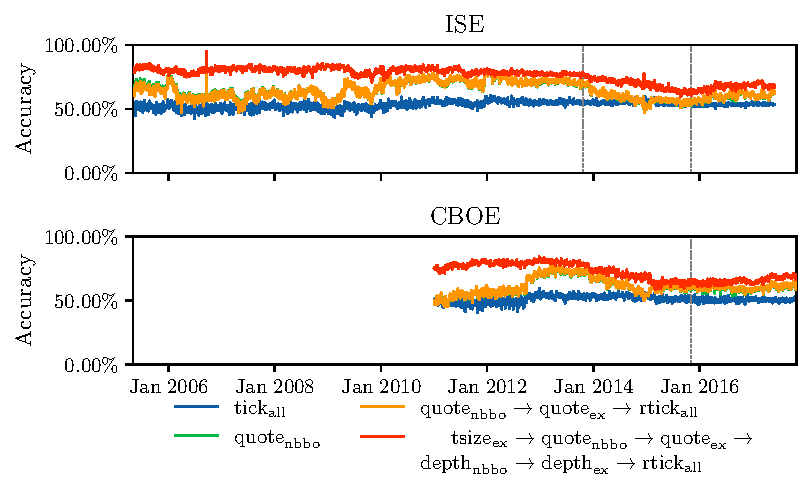
\includegraphics{classical-accuracies-over-time.pdf}
    \caption[Accuracy Of Rule-Based Classifiers On \glsentryshort{ISE} and \glsentryshort{CBOE} Over Time]{Accuracy of rule-based classifiers on \gls{ISE} and \gls{CBOE} sample over time. The dashed bar \myline{} indicates the beginning of a new subset based on the train-test split.}
    \label{fig:classical-accuracies-over-time}
\end{figure}

Aside from these high-level observations, we focus on three findings in greater detail.

\textbf{Finding 1: Accuracy of Basic Rules Is Downward-Biased by Missingness}

\todo{Add finding}

\textbf{Finding 2: Accuracy Comes From Depth}

\todo{Add finding}

\textbf{Finding 3: Fee Structures Affect Accuracy Over Time}

\todo{Add finding}

\begin{table}[ht]
    \centering
    \caption[Accuracies of Rule-Based Approaches On \glsentryshort{CBOE}]{This table shows the accuracy of common trade classification rules and their variations for option trades on \gls{CBOE} sample. Unclassifiable trades by the respective rule are assigned randomly as buy or sell. Hybrid methods are estimated using trade prices across all exchanges. We report the percentage of classifiable trades and the overall accuracy for subsets based on our train-test split and the entire dataset. The best rule is in bold.}
    \label{tab:cboe-classical}
    \begin{tabular}{lSSSS}
        \toprule
        {}                                     & {Coverage in \%}  & \multicolumn{3}{c}{Accuracy in \%}                                         \\ \cmidrule(lr){2-2}\cmidrule(lr){3-5}
        {Classification Rule}                  & {All}             & {Pre-Test}                         & {Test}            & {All}             \\\midrule
        $\operatorname{tick}_{\mathrm{ex}}$    & 91.4507           & 48.6156                            & 48.9969           & 48.7469           \\
        $\operatorname{rtick}_{\mathrm{ex}}$   & 90.2769           & 51.0857                            & 50.5432           & 50.8989           \\
        $\operatorname{quote}_{\mathrm{ex}}$   & 90.5150           & 62.6661                            & 62.0689           & 62.4605           \\
        $\operatorname{lr}_{\mathrm{ex}}$      & 99.7455           & 62.3106                            & 61.5831           & 62.0602           \\
        $\operatorname{rlr}_{\mathrm{ex}}$     & 99.4584           & 62.7035                            & 61.9898           & 62.4578           \\
        $\operatorname{emo}_{\mathrm{ex}}$     & 97.9601           & 49.3923                            & 48.6489           & 49.1364           \\
        $\operatorname{remo}_{\mathrm{ex}}$    & 97.3242           & 49.8883                            & 49.9529           & 49.9105           \\
        $\operatorname{clnv}_{\mathrm{ex}}$    & 98.4350           & 54.2644                            & 53.2492           & 53.9149           \\
        $\operatorname{rclnv}_{\mathrm{ex}}$   & 98.0358           & 55.1506                            & 54.5686           & 54.9502           \\\midrule
        $\operatorname{tick}_{\mathrm{all}}$   & 97.2135           & 51.4199                            & 50.4403           & 51.0827           \\
        $\operatorname{rtick}_{\mathrm{all}}$  & 96.0292           & 54.2521                            & 52.7056           & 53.7197           \\\midrule
        $\operatorname{quote}_{\mathrm{nbbo}}$ & 91.1772           & 61.3222                            & 59.8123           & 60.8024           \\
        $\operatorname{lr}_{\mathrm{nbbo}}$    & 99.7705           & 60.9503                            & 59.3730           & 60.4073           \\
        $\operatorname{rlr}_{\mathrm{nbbo}}$   & 99.6335           & 61.3095                            & 59.7608           & 60.7764           \\
        $\operatorname{emo}_{\mathrm{nbbo}}$   & 98.7186           & 51.6420                            & 51.6299           & 51.6378           \\
        $\operatorname{remo}_{\mathrm{nbbo}}$  & 98.3939           & 52.4847                            & 53.0736           & 52.6874           \\
        $\operatorname{clnv}_{\mathrm{nbbo}}$  & 98.8975           & 55.3058                            & 54.1294           & 54.9008           \\
        $\operatorname{rclnv}_{\mathrm{nbbo}}$ & 98.7000           & 56.3217                            & 55.4032           & 56.0055           \\\midrule
        $\operatorname{gsu}_{\mathrm{small}}$  & 99.7918           & 61.8938                            & 60.7464           & 61.4988           \\
        $\operatorname{gsu}_{\mathrm{large}}$  & \bfseries 99.9943 & \bfseries 74.6511                  & \bfseries 66.5176 & \bfseries 71.8510 \\\bottomrule
    \end{tabular}
\end{table}

We repeat the analysis on the \gls{CBOE} dataset in \cref{tab:cboe-classical} and observe a similar ranking to \cref{tab:ise-classical}. Overall, the performance of classical trade classification rules further diminishes or remains at a low level strengthening the need for alternative classifiers. Tick-based rules trail the performance of quote-based approaches, and the accuracy of hybrids varies with the dependence on the tick test. Different from the \gls{ISE} sample, the quote rule estimated on the \gls{NBBO}, $\operatorname{quote}_{\mathrm{nbbo}}$, leads to a lower performance than the quote rule applied to \gls{CBOE} quotes.
% Parts of this is due to the fact, that  $\operatorname{quote}_{\mathrm{nbbo}}$ achieves a considerably lower coverage of \SI{94.77}{\percent} compared to \SI{99.89}{\percent} in the \gls{ISE} sample, with fewer trades classified by the fallback criterion. In a filtered common sample, where trades are classified by both rules, performance is approximately similar. 
Again, $\operatorname{gsu}_{\mathrm{small}}$ and $\operatorname{gsu}_{\mathrm{large}}$ perform best, the strong outperformance does not carry over to the test set as depicted \cref{fig:classical-accuracies-over-time}.\footnote{Performance on \gls{CBOE} can be improved if the order of quote rules is reversed. For full combinatoric coverage see \textcite[][33]{grauerOptionTradeClassification2022}. To avoid overfitting the test set by classical rules, we keep the baseline constant following our reasoning from \cref{sec:hyperparameter-tuning}.}

\todo{Doesn't this contradict the hidden order idea of Grauer? Why are accuracies lower?}

Next, we test the supervised classifiers on the \gls{ISE}/\gls{CBOE} test sets, which prove to be a challenging test ground for rule-based classifiers as our results from above indicate.

\subsection{Results of Supervised
    Models}\label{sec:results-of-supervised-models}

We test the performance of our supervised models. We take the best configurations from \cref{sec:hyperparameter-tuning}, trained and tuned on the \gls{ISE} trade data, and evaluate their performance on the \gls{ISE} and \gls{CBOE} test sets. \cref{tab:results-supervised-ise-cboe} summarizes the results and benchmarks against state-of-the-art solutions from the literature.

\begin{table}[ht]
    \centering
    \caption[Accuracies of Supervised Approaches On \glsentryshort{CBOE} and \glsentryshort{ISE} Dataset]{This table reports the accuracy of supervised \glspl{GBRT} and Transformers for different feature combinations on the \gls{ISE} and \gls{CBOE} datasets. The improvement is estimated as the absolute change in accuracy between the classifier and the benchmark. For feature set classical, $\operatorname{gsu}_{\mathrm{small}}$ is the benchmark and otherwise $\operatorname{gsu}_{\mathrm{large}}$. Models are trained on the \gls{ISE} training set. The best classifier per dataset is in bold.}
    \label{tab:results-supervised-ise-cboe}
    \begin{tabular}{@{}llSSSSSS@{}}
        \toprule
                   &             & \multicolumn{2}{c}{FS Classical} & \multicolumn{2}{c}{FS Classical-Size} & \multicolumn{2}{c}{FS Option}                                                                 \\ \cmidrule(lr){3-4}\cmidrule(lr){5-6} \cmidrule(lr){7-8}
        Dataset    & Classifier  & {Acc. in \%}                     & {+/-}                                 & {Acc. in \%}                  & {+/-}              & {Acc. in \%}        & {+/-}              \\ \midrule
        \gls{ISE}  & \gls{GBRT}  & 63.668637                        & 3.620000                              & 72.343640                     & 4.730000           & \bfseries 74.120496 & \bfseries 6.510000 \\
                   & Transformer & \bfseries 63.783020              & \bfseries 3.730000                    & \bfseries 72.581107           & \bfseries 4.970000 & 73.921795           & 6.310000           \\ \addlinespace
        \gls{CBOE} & \gls{GBRT}  & 66.002029                        & 5.260000                              & 71.951794                     & 5.430000           & \bfseries 74.375033 & \bfseries 7.860000 \\
                   & Transformer & \bfseries 66.182348              & \bfseries 5.440000                    & \bfseries 72.153338           & \bfseries 5.640000 & 74.278318           & 7.760000           \\ \bottomrule
    \end{tabular}
\end{table}

Both model architectures consistently outperform their respective benchmarks on the \gls{ISE} and \gls{CBOE} datasets, achieving state-of-the-art performance in option trade classification with comparable data requirements. Thereby, Transformers dominate the \gls{ISE} sample when trained on trade prices and quotes reaching \SI{63.783020}{\percent}  in accuracy and \SI{66.18}{\percent} on the \gls{CBOE} sample outperforming previous approaches by \SI{3.730000}{\percent} and \SI{5.440000}{\percent}. Additional trade size features improve the accuracy to \SI{72.581107}{\percent} for the \gls{ISE} sample and \SI{72.153338}{\percent} for the \gls{CBOE} sample. Gradient boosting outperforms all other approaches when trained on additional option features.

While absolute improvements in accuracy over $\operatorname{gsu}_{\mathrm{small}}$ are modest on the smallest feature set, improvements are substantial for larger feature sets ranging between \SI{4.730000}{\percent} to \SI{7.860000}{\percent} over $\operatorname{gsu}_{\mathrm{large}}$. Specifically, the addition of trade size-related features positively contributes to the performance. We discuss feature importances in \cref{sec:feature-importance}.

The results can be enhanced through retraining on the validation set improving accuracies to \SI{76.162269}{\percent}, as documented in \cref{app:results-of-supervised-models-with-re-training}. In favour of conservative estimates, our models in the main text do not use this technique.

Visually, the performance differences between gradient boosting and transformers on the same feature sets are minor, consistent with previous studies \autocites{grinsztajnWhyTreebasedModels2022}{gorishniyRevisitingDeepLearning2021}. These studies conclude, generally for tabular modelling, that neither Transformers nor \gls{GBRT} are universally superior.


To formally test, whether differences between both classifiers are significant, we construct contingency tables and pair-wise compare predictions using McNemar's test \autocite[][153--157]{mcnemarNoteSamplingError1947}. We formulate the null hypothesis that both classifiers have the same error rate.
Conceptually similar \textcite[][267]{odders-whiteOccurrenceConsequencesInaccurate2000}, uses contingency tables of rule-based methods and true labels. Here, contingency tables are used to pair-wise compare the predictions of \gls{GBRT} against Transformers. We study the performance against the true label as part of the robustness checks.

\begin{table}[!h]
    \centering
    \sisetup{table-number-alignment=right, table-format=7.0}
    \caption[Contingency Tables of Supervised Classifiers On \glsentryshort{CBOE} and \glsentryshort{ISE} Dataset]{This table contains the contingency tables of the supervised classifiers on the \gls{CBOE} and \gls{ISE} test set for feature set classical, classical-size, and option. Cells sum the number of trades, correctly/falsely classified by both classifiers or one. Additionally, McNemar's test statistic $\chi^2$ and the associated $p$-value are reported.}
    \label{tab:contigency-supervised-classifiers}
    \begin{tabular}{@{}llSSSSSS@{}}
        \toprule
                                                                          &           & \multicolumn{2}{c}{{FS Classical}}                          & \multicolumn{2}{c}{{FS Classical-Size}}                      & \multicolumn{2}{c}{{FS Option}}                                                             \\
        \cmidrule(l){3-4}\cmidrule(l){5-6}\cmidrule(l){7-8}
        \multicolumn{2}{l}{{$\downarrow$ Trans.$\rightarrow$ \gls{GBRT}}} & {Correct} & {Wrong}                                                     & {Correct}                                                    & {Wrong}                                                     & {Correct} & {Wrong}           \\
        \midrule
        \gls{ISE}                                                         & Correct   & 5904530                                                     & 374201                                                       & 6790958                                                     & 343265    & 6722730 & 586719  \\
                                                                          & Wrong     & 385481                                                      & 3197364                                                      & 366683                                                      & 2360670   & 567124  & 1985003 \\         \addlinespace
                                                                          &           & \multicolumn{2}{l}{{$\chi^2$=\num{167.4593329840644}}}      & \multicolumn{2}{l}{{$\chi^2$=\num{772.3888073492707}}}       & \multicolumn{2}{l}{{$\chi^2$}=\num{332.73576734443077}}                                     \\
                                                                          &           & \multicolumn{2}{l}{{$p$-val.=\num{2.6552012527789754e-38}}} & \multicolumn{2}{l}{{$p$-val.=\num{5.437047807508087e-170}}}  & \multicolumn{2}{l}{{$p$-val.}=\num{2.4374791750246844e-74}}                                 \\
        \midrule
        \gls{CBOE}                                                        & Correct   & 8085066                                                     & 357404                                                       & 8701205                                                     & 502313    & 8746656 & 766824  \\
                                                                          & Wrong     & 380469                                                      & 3968289                                                      & 528093                                                      & 3059617   & 754453  & 2523295 \\         \addlinespace
                                                                          &           & \multicolumn{2}{l}{{$\chi^2$=\num{720.9209389691722}}}      & \multicolumn{2}{l}{{$\chi^2$=\num{644.9465948373747}}}       & \multicolumn{2}{l}{{$\chi^2$=\num{100.58450893558503}}}                                     \\
                                                                          &           & \multicolumn{2}{l}{{$p$-val.=\num{8.441178009879888e-159}}} & \multicolumn{2}{l}{{$p$-val.=\num{2.8062978547775803e-142}}} & \multicolumn{2}{l}{{$p$-val.=\num{1.1345159386344345e-23}}}                                 \\
        \bottomrule
    \end{tabular}
\end{table}

Based on the contingency tables in \cref{tab:contigency-supervised-classifiers}, we observe that both models share a large portion of trades, for which both classifiers agree.\footnote{Through summation of correct classifications of one classifier divided by the matrix sum, one obtains the accuracy from \cref{tab:results-supervised-ise-cboe}. Consider the first entry, e.g., $(\num{5904530}+\num{374201}) / (\num{5904530} + \num{374201} + \num{385481} + \num{3197364}) \approx \num{0.63668637}$.} For larger feature sets, the share of trades correctly classified by one classifier grows, while the number of jointly correctly classified trades plateaus. This can be an indication, that both models learn specific patterns and excel in different trades. The performance differences between classifiers are statistically significant for at the \SI{1}{\percent}. The null hypothesis can be rejected.

Contrary to the expectation, the performance improvements are highest for the \gls{CBOE} dataset, despite the models being trained on \gls{ISE} data. Part of this is due to a weaker benchmark performance, but also due to the stronger accuracy of classifiers on the smallest and mid-sized feature sets. One would expect a degradation between sets, assuming exchange-specific trading patterns and requiring exploration in greater detail.

\textbf{Finding 4: Foo Affect Classifier Performance}

\todo{Formulate finding.}

% \begin{figure}[!h]
%     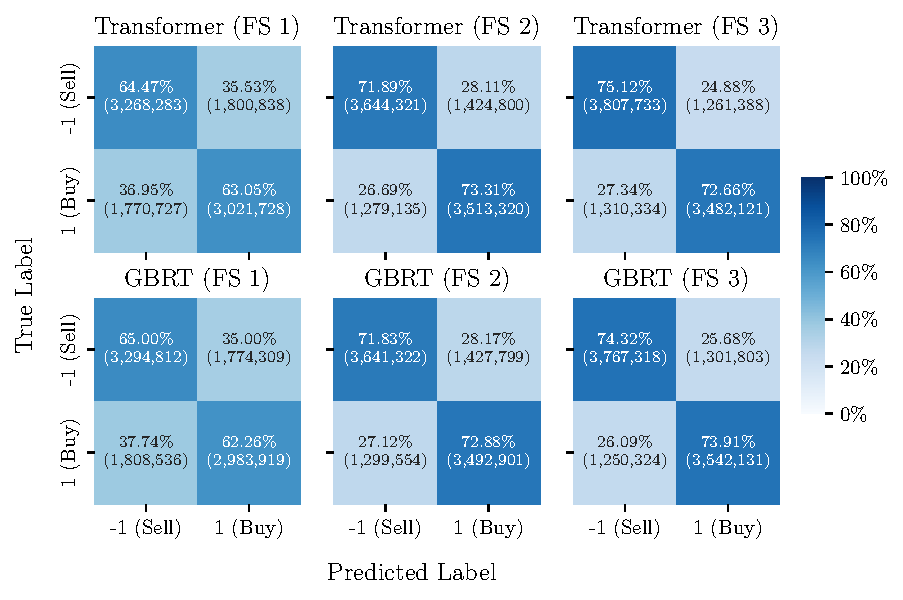
\includegraphics{confusion_matrix_ise.pdf}
%     \caption[Confusion Matrices Of Supervised Classifiers On \gls{ISE} Data Set]{tbd}
%     \label{fig:confusion-matrix-supervised-ise}
% \end{figure}

In summary, our supervised methods establish a new state-of-the-art in option trade classification. Our approach achieves full coverage and outperforms all previously reported classification rules in terms of accuracy. We perform robustness checks in \cref{sec:robustness-checks} to verify performance is consistent across sub-samples.

\subsection{Results of Semi-Supervised
    Models}\label{sec:results-of-semi-supervised-models}

We compare the performance of pre-trained Transformers and self-trained gradient-boosting on the \gls{ISE} and \gls{CBOE} test set. Results are reported in \cref{tab:results-semi-supervised-ise-cboe}.

\begin{table}[ht]
    \centering
    \caption[Accuracies of Semi-Supervised Approaches On \glsentryshort{CBOE} and \glsentryshort{ISE} Dataset]{This table reports the accuracy of semi-supervised \glspl{GBRT} and Transformers for different feature combinations on the \gls{ISE} and \gls{CBOE} datasets. The improvement is estimated as the absolute change in accuracy between the classifier and the benchmark. For feature set classical, $\operatorname{gsu}_{\mathrm{small}}$ is the benchmark and otherwise $\operatorname{gsu}_{\mathrm{large}}$. Models are trained on the \gls{ISE} training set. The best classifier per dataset is in bold.}
    \label{tab:results-semi-supervised-ise-cboe}
    \begin{tabular}{@{}llSSSSSS@{}}
        \toprule
                   &             & \multicolumn{2}{c}{FS Classical} & \multicolumn{2}{c}{FS Classical-Size} & \multicolumn{2}{c}{FS Option}                                      \\ \cmidrule(lr){3-4}\cmidrule(lr){5-6} \cmidrule(lr){7-8}
        Dataset    & Classifier  & {Acc. in \%}                     & {+/-}                                 & {Acc. in \%}                  & {+/-}    & {Acc. in \%} & {+/-}    \\ \midrule
        \gls{ISE}  & \gls{GBRT}  & 63.397514                        & 3.350000                              & 72.156489                     & 4.550000 & 73.536644    & 5.930000 \\
                   & Transformer &                                  &                                       &                               &          &              &          \\ \addlinespace
        \gls{CBOE} & \gls{GBRT}  & 66.189454                        & 5.440000                              & 71.922680                     & 5.410000 & 73.953322    & 7.440000 \\
                   & Transformer &                                  &                                       &                               &          &              &          \\ \bottomrule
    \end{tabular}
\end{table}

Identical to the supervised case, our models consistently outperform their respective benchmarks. Gradient boosting with self-training surpasses $\operatorname{gsu}_{\mathrm{small}}$ by \SI{3.350000}{\percent} on \gls{ISE} and \SI{5.440000}{\percent} on \gls{CBOE} in accuracy. Improvements for larger feature sets over $\operatorname{gsu}_{\mathrm{large}}$ are marginally lower to the supervised model and range between \SI{4.550000}{\percent} and \SI{7.440000}{\percent}.

The results do not support the hypothesis, that adding unlabelled trades into the training corpus improves generalisation performance of the classifier. We explore this finding in detail.

\textbf{Finding 5: Unlabelled Trades Provide Poor Guidance}

\todo{formulate finding}

\begin{table}[!h]
    \centering
    \sisetup{table-number-alignment=right, table-format=7.0}
    \caption[Contingency Tables of Semi-Supervised Classifiers On \glsentryshort{CBOE} and \glsentryshort{ISE} Dataset]{This table contains the contingency tables of the semi-supervised classifiers on the \gls{CBOE} and \gls{ISE} test set for feature set classical, classical-size, and option. Cells sum the number of trades, correctly/falsely classified by both classifiers or one. Additionally, McNemar's test statistic $\chi^2$ and the associated $p$-value are reported.}
    \label{tab:contigency-semi-supervised-classifiers}
    \begin{tabular}{@{}llSSSSSS@{}}
        \toprule
                                                                          &           & \multicolumn{2}{c}{{FS Classical}} & \multicolumn{2}{c}{{FS Classical-Size}} & \multicolumn{2}{c}{{FS Option}}                         \\
        \cmidrule(l){3-4}\cmidrule(l){5-6}\cmidrule(l){7-8}
        \multicolumn{2}{l}{{$\downarrow$ Trans.$\rightarrow$ \gls{GBRT}}} & {Correct} & {Wrong}                            & {Correct}                               & {Wrong}                         & {Correct} & {Wrong}   \\
        \midrule
        \gls{ISE}                                                         & Correct   &                                    &                                         &                                 &           &         & \\
                                                                          & Wrong     &                                    &                                         &                                 &           &         & \\         \addlinespace
                                                                          &           & \multicolumn{2}{l}{{$\chi^2$=}}    & \multicolumn{2}{l}{{$\chi^2$=}}         & \multicolumn{2}{l}{{$\chi^2$}=}                         \\
                                                                          &           & \multicolumn{2}{l}{{$p$-val.=}}    & \multicolumn{2}{l}{{$p$-val.=}}         & \multicolumn{2}{l}{{$p$-val.}=}                         \\
        \midrule
        \gls{CBOE}                                                        & Correct   &                                    &                                         &                                 &           &         & \\
                                                                          & Wrong     &                                    &                                         &                                 &           &         & \\         \addlinespace
                                                                          &           & \multicolumn{2}{l}{{$\chi^2$=}}    & \multicolumn{2}{l}{{$\chi^2$=}}         & \multicolumn{2}{l}{{$\chi^2$=}}                         \\
                                                                          &           & \multicolumn{2}{l}{{$p$-val.=}}    & \multicolumn{2}{l}{{$p$-val.=}}         & \multicolumn{2}{l}{{$p$-val.=}}                         \\
        \bottomrule
    \end{tabular}
\end{table}

To summarize, despite the significantly higher training costs, semi-supervised variants do not provide better generalisation performance than supervised approaches. We subsequently evaluate if semi-supervised learning improves robustness, if not performance.


\subsection{Robustness of Results}\label{sec:robustness-checks}

\todo{Again, results are not 100 \% comparaable due to grouping.}
\todo{Compare improvements with other works. Improvments much greater than ronen et al. }

\textbf{Gradient Boosting}

\begin{table}[ht!]
    \centering
    \caption[short-diff-ise-supervised-test-gbm]{long-diff-ise-supervised-test-gbm}
    \label{tab:diff-ise_supervised_test}
    \begin{tabular}{lSSSSSS@{}}
        \toprule
        {}                       & \multicolumn{2}{c}{FS Classical} & \multicolumn{2}{c}{FS Classical-Size} & \multicolumn{2}{c}{FS Option}                                        \\ \cmidrule(lr){2-3}\cmidrule(lr){4-5}\cmidrule(lr){6-7}
        {}                       & {Acc. in \%}                     & {+/-}                                 & {Acc. in \%}                  & {+/-}     & {Acc. in \%} & {+/-}     \\\midrule
        \multicolumn{7}{l}{ Option Type}                                                                                                                                           \\
        \tabindent  C            & 62.890486                        & 3.720000                              & 71.884647                     & 4.480000  & 73.647971    & 6.240000  \\
        \tabindent  P            & 64.557394                        & 3.500000                              & 72.867874                     & 5.020000  & 74.660185    & 6.820000  \\
        \cmidrule(rl){1-7}
        \multicolumn{7}{l}{ Security Type}                                                                                                                                         \\
        \tabindent  Index option & 56.345043                        & -1.460000                             & 57.474458                     & -1.020000 & 58.649239    & 0.150000  \\
        \tabindent Others        & 68.399095                        & 2.870000                              & 76.369535                     & 5.790000  & 77.590573    & 7.010000  \\
        \tabindent Stock Option  & 61.877752                        & 4.000000                              & 70.946999                     & 4.400000  & 72.956919    & 6.410000  \\
        \cmidrule(rl){1-7}
        \multicolumn{7}{l}{ Trade Size}                                                                                                                                            \\
        \tabindent (0,1]         & 61.892029                        & 3.350000                              & 72.564793                     & 3.390000  & 74.245655    & 5.070000  \\
        \tabindent  (1,3]        & 62.473959                        & 4.020000                              & 72.965377                     & 3.680000  & 74.857610    & 5.570000  \\
        \tabindent  (3,5]        & 62.696932                        & 3.890000                              & 72.755628                     & 3.360000  & 74.647279    & 5.250000  \\
        \tabindent  (5,11]       & 65.928967                        & 3.380000                              & 71.752039                     & 8.080000  & 73.450299    & 9.780000  \\
        \tabindent  >11          & 67.310266                        & 3.640000                              & 71.337373                     & 6.380000  & 73.145472    & 8.190000  \\
        \cmidrule(rl){1-7}
        \multicolumn{7}{l}{ Year}                                                                                                                                                  \\
        \tabindent 2015          & 60.446922                        & 4.050000                              & 69.000296                     & 5.210000  & 71.512360    & 7.730000  \\
        \tabindent  2016         & 63.736474                        & 3.560000                              & 72.555638                     & 5.030000  & 74.290527    & 6.770000  \\
        \tabindent  2017         & 64.596306                        & 3.610000                              & 72.977560                     & 3.870000  & 74.604216    & 5.500000  \\
        \cmidrule(rl){1-7}
        \multicolumn{7}{l}{ Time To Maturity}                                                                                                                                      \\
        \tabindent  <= 1         & 64.458297                        & 3.580000                              & 72.756774                     & 5.240000  & 74.604553    & 7.090000  \\
        \tabindent  (1-2]        & 64.612677                        & 3.800000                              & 72.869099                     & 4.300000  & 73.947396    & 5.370000  \\
        \tabindent (2-3]         & 63.015912                        & 3.110000                              & 71.743691                     & 3.460000  & 72.997282    & 4.710000  \\
        \tabindent  (3-6]        & 61.788369                        & 3.640000                              & 71.288086                     & 3.430000  & 72.750293    & 4.890000  \\
        \tabindent  (6-12]       & 61.911555                        & 3.990000                              & 71.199996                     & 3.310000  & 73.130453    & 5.240000  \\
        \tabindent  > 12         & 55.126547                        & 3.830000                              & 68.572852                     & 3.540000  & 72.004951    & 6.980000  \\
        \cmidrule(rl){1-7}
        \multicolumn{7}{l}{ Moneyness}                                                                                                                                             \\
        \tabindent  <= 0.7       & 65.531247                        & 3.790000                              & 71.917341                     & 7.520000  & 72.307517    & 7.910000  \\
        \tabindent  (0.7-0.9]    & 67.642270                        & 3.670000                              & 74.254665                     & 5.960000  & 75.433765    & 7.140000  \\
        \tabindent  (0.9-1.1]    & 64.059687                        & 3.530000                              & 72.975308                     & 4.400000  & 74.457482    & 5.880000  \\
        \tabindent  (1.1-1.3]    & 54.294722                        & 4.040000                              & 66.220667                     & 4.190000  & 70.375579    & 8.350000  \\
        \tabindent  > 1.3        & 52.623795                        & 3.770000                              & 63.075529                     & 2.870000  & 70.489510    & 10.280000 \\
        \cmidrule(rl){1-7}
        \multicolumn{7}{l}{ Proximity To Quotes}                                                                                                                                   \\
        \tabindent  At Mid       & 62.644890                        & 5.490000                              & 72.164951                     & 4.020000  & 74.685118    & 6.540000  \\
        \tabindent  Inside       & 62.605233                        & 2.160000                              & 68.301819                     & 3.800000  & 70.295127    & 5.790000  \\
        \tabindent  At Quotes    & 67.828443                        & 7.860000                              & 86.667541                     & 8.450000  & 87.313763    & 9.100000  \\
        \tabindent  Outside      & 61.350064                        & -5.430000                             & 61.846608                     & -3.070000 & 64.034087    & -0.890000 \\
        \tabindent  Unknown      & 78.638385                        & 2.230000                              & 78.275744                     & 1.870000  & 78.816285    & 2.410000  \\
        \cmidrule(rl){1-7}
        \multicolumn{7}{l}{ All}                                                                                                                                                   \\
        \tabindent  All          & 63.668637                        & 3.620000                              & 72.343640                     & 4.730000  & 74.120496    & 6.510000  \\
        \bottomrule
    \end{tabular}
\end{table}



\begin{table}[h!]
    \centering
    \caption[short-diff-cboe-transfer-test]{long-diff-cboe-gbm-tbd}
    \label{tab:diff-cboe_transfer-gbm}
    \begin{tabular}{lSSSSSS@{}}
        \toprule
        {}                      & \multicolumn{2}{c}{FS Classical} & \multicolumn{2}{c}{FS Classical-Size} & \multicolumn{2}{c}{FS Option}                                        \\ \cmidrule(lr){2-3}\cmidrule(lr){4-5}\cmidrule(lr){6-7}
        {}                      & {Acc. in \%}                     & {+/-}                                 & {Acc. in \%}                  & {+/-}     & {Acc. in \%} & {+/-}     \\\midrule
        \multicolumn{7}{l}{ Option Type}                                                                                                                                          \\
        \tabindent C            & 65.505083                        & 5.370000                              & 71.707057                     & 5.770000  & 74.283388    & 8.350000  \\
        \tabindent P            & 66.597419                        & 5.120000                              & 72.245014                     & 5.030000  & 74.484832    & 7.270000  \\
        \cmidrule(rl){1-7}
        \multicolumn{7}{l}{Security Type}                                                                                                                                         \\
        \tabindent Index Option & 60.365562                        & 7.070000                              & 67.298912                     & 0.850000  & 72.394792    & 5.940000  \\
        \tabindent Others       & 69.054857                        & 4.420000                              & 74.137168                     & 5.210000  & 75.534837    & 6.610000  \\
        \tabindent Stock Option & 65.293961                        & 5.420000                              & 71.506273                     & 5.980000  & 74.089988    & 8.570000  \\
        \cmidrule(rl){1-7}
        \multicolumn{7}{l}{ Trade Size}                                                                                                                                           \\
        \tabindent (0,1]        & 62.831155                        & 5.860000                              & 70.756340                     & 6.780000  & 73.423543    & 9.450000  \\
        \tabindent (1,3]        & 64.895723                        & 5.200000                              & 71.318816                     & 6.330000  & 73.634574    & 8.640000  \\
        \tabindent (3,5]        & 65.549362                        & 5.060000                              & 71.956770                     & 5.620000  & 74.174579    & 7.840000  \\
        \tabindent(5,11]        & 66.577620                        & 5.150000                              & 71.566680                     & 5.170000  & 74.143799    & 7.750000  \\
        \tabindent >11          & 71.136074                        & 4.750000                              & 74.549126                     & 2.830000  & 76.765762    & 5.050000  \\
        \cmidrule(rl){1-7}
        \multicolumn{7}{l}{Year}                                                                                                                                                  \\                                                                                                                                        \\
        \tabindent 2015         & 65.689585                        & 4.460000                              & 71.445193                     & 6.400000  & 74.317847    & 9.270000  \\
        \tabindent 2016         & 65.579978                        & 5.350000                              & 71.638148                     & 6.430000  & 74.178699    & 8.970000  \\
        \tabindent 2017         & 66.491658                        & 5.250000                              & 72.349451                     & 4.250000  & 74.591947    & 6.500000  \\
        \cmidrule(rl){1-7}
        \multicolumn{7}{l}{ Time To Maturity}                                                                                                                                     \\
        \tabindent <= 1         & 66.863272                        & 4.940000                              & 72.005520                     & 5.140000  & 74.272153    & 7.410000  \\
        \tabindent (1-2]        & 67.553775                        & 5.590000                              & 72.584599                     & 5.170000  & 75.237684    & 7.820000  \\
        \tabindent (2-3]        & 66.061857                        & 5.770000                              & 72.349461                     & 5.110000  & 74.713903    & 7.480000  \\
        \tabindent (3-6]        & 65.007308                        & 5.950000                              & 72.855935                     & 6.220000  & 75.086134    & 8.450000  \\
        \tabindent (6-12]       & 64.184403                        & 5.600000                              & 71.908786                     & 6.200000  & 74.389885    & 8.690000  \\
        \tabindent > 12         & 56.065976                        & 5.380000                              & 66.802260                     & 7.160000  & 71.092148    & 11.450000 \\
        \cmidrule(rl){1-7}
        \multicolumn{7}{l}{ Moneyness}                                                                                                                                            \\
        \tabindent <= 0.7       & 65.722320                        & 5.400000                              & 72.842929                     & 3.880000  & 75.645703    & 6.680000  \\
        \tabindent (0.7-0.9]    & 66.272446                        & 5.460000                              & 72.187575                     & 5.130000  & 74.768887    & 7.710000  \\
        \tabindent (0.9-1.1]    & 66.977290                        & 5.190000                              & 72.619255                     & 5.420000  & 74.739508    & 7.540000  \\
        \tabindent (1.1-1.3]    & 58.197013                        & 5.020000                              & 66.153817                     & 7.100000  & 69.833429    & 10.780000 \\
        \tabindent > 1.3        & 56.958403                        & 5.890000                              & 64.569317                     & 6.580000  & 70.478616    & 12.490000 \\
        \cmidrule(rl){1-7}
        \multicolumn{7}{l}{ Proximity To Quotes}                                                                                                                                  \\
        \tabindent At Mid       & 60.688727                        & 6.950000                              & 67.528635                     & 4.080000  & 69.104800    & 5.660000  \\
        \tabindent Inside       & 68.822448                        & 3.030000                              & 71.987785                     & 6.150000  & 73.698272    & 7.860000  \\
        \tabindent At Quotes    & 54.187224                        & 16.010000                             & 74.756821                     & 2.410000  & 81.426352    & 9.080000  \\
        \tabindent Outside      & 70.719978                        & -4.200000                             & 70.369607                     & -1.560000 & 69.648255    & -2.280000 \\
        \tabindent Unknown      & 83.771336                        & 1.110000                              & 83.608778                     & 0.950000  & 84.213854    & 1.550000  \\
        \cmidrule(rl){1-7}
        \multicolumn{7}{l}{ All}                                                                                                                                                  \\
        \tabindent All          & 66.002029                        & 5.260000                              & 71.951794                     & 5.430000  & 74.375033    & 7.860000  \\
        \bottomrule
    \end{tabular}
\end{table}


\textbf{FT-Transformer}

\begin{table}[h!]
    \centering
    \caption[short-diff-ise-supervised-test-fttransformer]{long-diff-ise-supervised-test-fttransformer}
    \label{tab:diff-ise_supervised-test}
    \begin{tabular}{lSSSSSS@{}}
        \toprule
        {}                      & \multicolumn{2}{c}{FS Classical} & \multicolumn{2}{c}{FS Classical-Size} & \multicolumn{2}{c}{FS Option}                                        \\ \cmidrule(lr){2-3}\cmidrule(lr){4-5}\cmidrule(lr){6-7}
        {}                      & {Acc. in \%}                     & {+/-}                                 & {Acc. in \%}                  & {+/-}     & {Acc. in \%} & {+/-}     \\\midrule
        \multicolumn{7}{l}{ Option Type}                                                                                                                                          \\
        \tabindent C            & 62.991514                        & 3.820000                              & 72.099064                     & 4.690000  & 73.484904    & 6.080000  \\
        \tabindent P            & 64.687031                        & 3.630000                              & 73.131667                     & 5.290000  & 74.420786    & 6.580000  \\
        \cmidrule(rl){1-7}
        \multicolumn{7}{l}{ Security Type}                                                                                                                                        \\
        \tabindent Index option & 56.519890                        & -1.290000                             & 58.457380                     & -0.040000 & 58.641678    & 0.140000  \\
        \tabindent Others       & 68.443599                        & 2.920000                              & 76.549050                     & 5.970000  & 77.590109    & 7.010000  \\
        \tabindent Stock option & 62.019384                        & 4.140000                              & 71.196166                     & 4.650000  & 72.674763    & 6.120000  \\
        \cmidrule(rl){1-7}
        \multicolumn{7}{l}{ Trade Size}                                                                                                                                           \\
        \tabindent (0,1]        & 62.127137                        & 3.590000                              & 72.877007                     & 3.710000  & 73.967386    & 4.800000  \\
        \tabindent (1,3]        & 62.654716                        & 4.200000                              & 73.321548                     & 4.040000  & 74.721308    & 5.440000  \\
        \tabindent (3,5]        & 62.839285                        & 4.030000                              & 73.161769                     & 3.770000  & 74.715927    & 5.320000  \\
        \tabindent (5,11]       & 65.756057                        & 3.200000                              & 71.877263                     & 8.210000  & 73.441354    & 9.770000  \\
        \tabindent >11          & 67.380602                        & 3.710000                              & 71.237293                     & 6.280000  & 72.584805    & 7.630000  \\
        \cmidrule(rl){1-7}
        \multicolumn{7}{l}{ Year}                                                                                                                                                 \\
        \tabindent 2015         & 60.620179                        & 4.220000                              & 69.609946                     & 5.820000  & 71.861077    & 8.070000  \\
        \tabindent 2016         & 63.851905                        & 3.680000                              & 72.798245                     & 5.270000  & 74.138951    & 6.620000  \\
        \tabindent 2017         & 64.688426                        & 3.700000                              & 73.077731                     & 3.970000  & 74.111711    & 5.010000  \\
        \cmidrule(rl){1-7}
        \multicolumn{7}{l}{ Time To Maturity}                                                                                                                                     \\
        \tabindent <= 1         & 64.546416                        & 3.670000                              & 72.976628                     & 5.460000  & 74.450445    & 6.930000  \\
        \tabindent (1-2]        & 64.736461                        & 3.930000                              & 73.043470                     & 4.470000  & 73.692560    & 5.120000  \\
        \tabindent(2-3]         & 63.152545                        & 3.250000                              & 72.063690                     & 3.780000  & 72.896064    & 4.610000  \\
        \tabindent (3-6]        & 61.887659                        & 3.740000                              & 71.531191                     & 3.670000  & 72.287641    & 4.420000  \\
        \tabindent (6-12]       & 62.021518                        & 4.100000                              & 71.325950                     & 3.430000  & 72.466903    & 4.570000  \\
        \tabindent > 12         & 55.669126                        & 4.380000                              & 69.313656                     & 4.290000  & 72.282466    & 7.250000  \\
        \cmidrule(rl){1-7}
        \multicolumn{7}{l}{ Moneyness}                                                                                                                                            \\
        \tabindent <= 0.7       & 65.196444                        & 3.460000                              & 71.762641                     & 7.370000  & 71.689001    & 7.290000  \\
        \tabindent (0.7-0.9]    & 67.618182                        & 3.650000                              & 74.318808                     & 6.030000  & 74.876535    & 6.580000  \\
        \tabindent (0.9-1.1]    & 64.141472                        & 3.610000                              & 73.115683                     & 4.540000  & 74.236648    & 5.660000  \\
        \tabindent (1.1-1.3]    & 54.943206                        & 4.690000                              & 67.505754                     & 5.480000  & 70.929706    & 8.900000  \\
        \tabindent > 1.3        & 53.468351                        & 4.620000                              & 64.293219                     & 4.080000  & 71.424038    & 11.210000 \\
        \cmidrule(rl){1-7}
        \multicolumn{7}{l}{ Proximity To Quotes}                                                                                                                                  \\
        \tabindent At Mid       & 62.490146                        & 5.340000                              & 72.138236                     & 3.990000  & 74.022892    & 5.870000  \\
        \tabindent Inside       & 62.566010                        & 2.120000                              & 68.807735                     & 4.300000  & 70.429973    & 5.930000  \\
        \tabindent At Quotes    & 68.608870                        & 8.640000                              & 86.087938                     & 7.870000  & 86.165327    & 7.950000  \\
        \tabindent Outside      & 63.228880                        & -3.550000                             & 63.792525                     & -1.130000 & 65.610951    & 0.690000  \\
        \tabindent Unknown      & 78.268902                        & 1.860000                              & 77.824153                     & 1.420000  & 78.522066    & 2.110000  \\
        \cmidrule(rl){1-7}
        \multicolumn{7}{l}{ All}                                                                                                                                                  \\
        \tabindent All          & 63.783020                        & 3.730000                              & 72.581107                     & 4.970000  & 73.921795    & 6.310000  \\
        \bottomrule
    \end{tabular}
\end{table}

\begin{table}[h!]
    \centering
    \caption[short-diff-cboe-transfer-test-fttransformer]{long-diff-cboe-transfer-test-fttransformer}
    \label{tab:diff-cboe_transfer_test}
    \begin{tabular}{lSSSSSS@{}}
        \toprule
        {}                      & \multicolumn{2}{c}{FS Classical} & \multicolumn{2}{c}{FS Classical-Size} & \multicolumn{2}{c}{FS Option}                                       \\ \cmidrule(lr){2-3}\cmidrule(lr){4-5}\cmidrule(lr){6-7}
        {}                      & {Acc. in \%}                     & {+/-}                                 & {Acc. in \%}                  & {+/-}    & {Acc. in \%} & {+/-}     \\\midrule
        \multicolumn{7}{l}{ Option Type}                                                                                                                                         \\
        \tabindent C            & 65.628907                        & 5.490000                              & 71.945453                     & 6.010000 & 74.579113    & 8.640000  \\
        \tabindent P            & 66.845425                        & 5.370000                              & 72.402406                     & 5.190000 & 73.917935    & 6.700000  \\
        \cmidrule(rl){1-7}
        \multicolumn{7}{l}{ Security Type}                                                                                                                                       \\
        \tabindent Index option & 61.207800                        & 7.910000                              & 67.170125                     & 0.720000 & 69.051358    & 2.600000  \\
        \tabindent Others       & 69.266211                        & 4.630000                              & 74.427252                     & 5.500000 & 75.859396    & 6.940000  \\
        \tabindent Stock option & 65.395694                        & 5.520000                              & 71.703855                     & 6.180000 & 74.141068    & 8.620000  \\
        \cmidrule(rl){1-7}
        \multicolumn{7}{l}{ Trade Size}                                                                                                                                          \\
        \tabindent (0,1]        & 63.135782                        & 6.170000                              & 71.074930                     & 7.100000 & 73.362654    & 9.380000  \\
        \tabindent (1,3]        & 64.993995                        & 5.300000                              & 71.513064                     & 6.520000 & 73.846381    & 8.860000  \\
        \tabindent (3,5]        & 65.605000                        & 5.110000                              & 72.070498                     & 5.730000 & 74.237799    & 7.900000  \\
        \tabindent (5,11]       & 66.701471                        & 5.280000                              & 71.890991                     & 5.490000 & 73.979636    & 7.580000  \\
        \tabindent >11          & 71.378727                        & 4.990000                              & 74.552019                     & 2.840000 & 76.246445    & 4.530000  \\
        \cmidrule(rl){1-7}
        \multicolumn{7}{l}{ Year}                                                                                                                                                \\
        \tabindent 2015         & 65.830149                        & 4.600000                              & 71.843643                     & 6.800000 & 74.755266    & 9.710000  \\
        \tabindent 2016         & 65.786999                        & 5.560000                              & 71.935076                     & 6.720000 & 74.353864    & 9.140000  \\
        \tabindent 2017         & 66.648330                        & 5.410000                              & 72.424788                     & 4.330000 & 74.138831    & 6.040000  \\
        \cmidrule(rl){1-7}
        \multicolumn{7}{l}{ Time To Maturity}                                                                                                                                    \\
        \tabindent <= 1         & 66.927563                        & 5.000000                              & 72.081695                     & 5.220000 & 74.167407    & 7.310000  \\
        \tabindent (1-2]        & 67.642166                        & 5.680000                              & 72.576488                     & 5.160000 & 74.914699    & 7.500000  \\
        \tabindent (2-3]        & 66.550561                        & 6.250000                              & 72.383470                     & 5.150000 & 73.512089    & 6.280000  \\
        \tabindent (3-6]        & 65.257500                        & 6.200000                              & 73.243404                     & 6.610000 & 75.241041    & 8.610000  \\
        \tabindent (6-12]       & 64.630833                        & 6.050000                              & 72.430785                     & 6.730000 & 74.759232    & 9.050000  \\
        \tabindent > 12         & 56.949258                        & 6.270000                              & 68.451314                     & 8.810000 & 71.975430    & 12.340000 \\
        \cmidrule(rl){1-7}
        \multicolumn{7}{l}{ Moneyness}                                                                                                                                           \\
        \tabindent <= 0.7       & 65.747181                        & 5.420000                              & 72.938769                     & 3.980000 & 75.030310    & 6.070000  \\
        \tabindent (0.7-0.9]    & 66.501088                        & 5.690000                              & 72.160406                     & 5.100000 & 73.928341    & 6.870000  \\
        \tabindent (0.9-1.1]    & 67.105536                        & 5.320000                              & 72.698844                     & 5.500000 & 74.754866    & 7.560000  \\
        \tabindent (1.1-1.3]    & 58.732468                        & 5.550000                              & 67.827369                     & 8.770000 & 70.847531    & 11.790000 \\
        \tabindent > 1.3        & 57.597394                        & 6.530000                              & 66.397443                     & 8.400000 & 71.088957    & 13.100000 \\
        \cmidrule(rl){1-7}
        \multicolumn{7}{l}{ Proximity To Quotes}                                                                                                                                 \\
        \tabindent At Mid       & 60.688727                        & 6.950000                              & 67.528635                     & 4.080000 & 69.104800    & 5.660000  \\
        \tabindent Inside       & 68.679525                        & 2.890000                              & 72.284311                     & 6.440000 & 73.930387    & 8.090000  \\
        \tabindent At Quotes    & 56.479734                        & 18.300000                             & 74.815580                     & 2.470000 & 79.999142    & 7.650000  \\
        \tabindent Outside      & 73.145095                        & -1.770000                             & 72.581753                     & 0.650000 & 71.908491    & -0.020000 \\
        \tabindent Unknown      & 83.807460                        & 1.150000                              & 83.220446                     & 0.560000 & 83.491375    & 0.830000  \\
        \cmidrule(rl){1-7}
        \multicolumn{7}{l}{ All}                                                                                                                                                 \\
        \tabindent All          & 66.182348                        & 5.440000                              & 72.153338                     & 5.640000 & 74.278318    & 7.760000  \\
        \bottomrule
    \end{tabular}
\end{table}

\todo{When the analysis was repeated using only the Lee and Radhakrishna subsample, the results were equally as strong or stronger, with two exceptions. Using their subsample, time between transactions is no longer a statistically signi"cant determinant of misclassi"cation and large trades are misclassi"ed slightly more frequently than small trades (odderswhite)}
\todo{Our focus is on ... rules.}
\todo{Improvements are particularily high for trades that are notourisly hard to classify by classical trade classification algorithms.}

\clearpage

\subsection{Feature Importance}\label{sec:feature-importance}

\textbf{Sage Values}

\begin{figure}[h!]
    \centering
    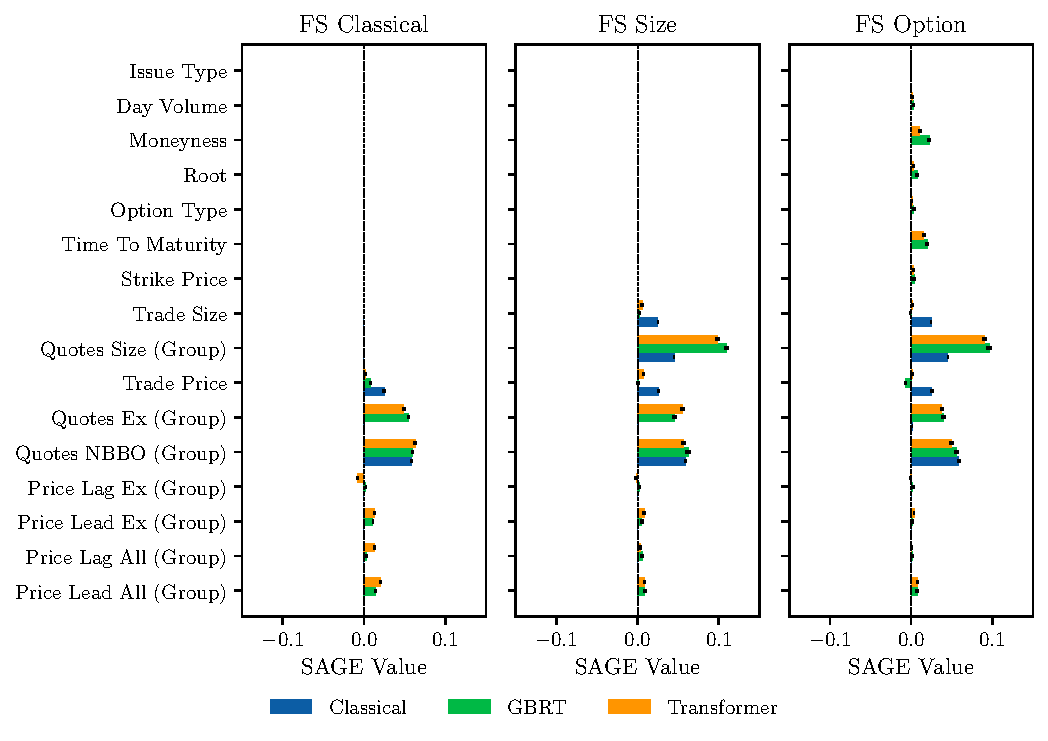
\includegraphics[width=1\textwidth]{sage-importances.pdf}
    \caption[tbd]{tbd}
    \label{fig:sage-importances}
\end{figure}

\textbf{Attention Maps}

\begin{figure}[h!]
    \centering
    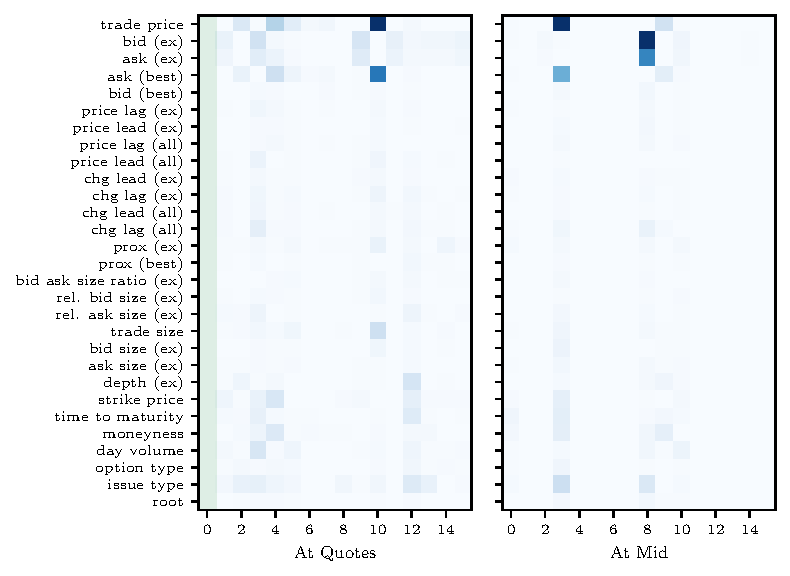
\includegraphics[width=1\textwidth]{attention_maps_ise_quotes_mid.pdf}
    \caption[tbd]{tbd}
    \label{fig:attention-maps-ise}
\end{figure}

\textbf{Categorical Embeddings}

For the Transformer we know from \cref{sec:token-embeddings}, that embeddings can capture similarities by arranging related objects closer in embedding space. Visualising the learnt embeddings gives insights into the model.

The embeddings are queried from the feature tokenizer in FT-Transformer. The similarity between embeddings is measured by cosine distance in embedding space. The high-dimensional embeddings are then projected into 2D space using $t$-SNE \autocite{vandermaatenVisualizingDataUsing2008}. As straightforward to interpret, we focus our analysis on the underlying, but note, that it applies to any numerical and categorical embeddings.

Figure \cref{fig:categorical-embeddings} illustrates the embeddings exemplary for SPDR S\&P 500 Trust ($\mathtt{SPY}$) and JPMorgan Chase \& Co ($\mathtt{JPM}$).\footnote{As our analysis is condensed to two underlyings, we encourage the reader to use our interactive visualisation for further exploration. Accessible here \url{https://wandb.ai/fbv/thesis/runs/3cirr6nk}.} For SPY \todo{Graphically, ... wait for list of underlyings. What was not input to the model?}. For JPM \todo{Visually performs ... wait for the list of underlyings}

\begin{figure}[h!]
    \subfloat[Most Similar Embeddings to $\mathtt{SPY}$\label{fig:cat-embeddings-spy}]{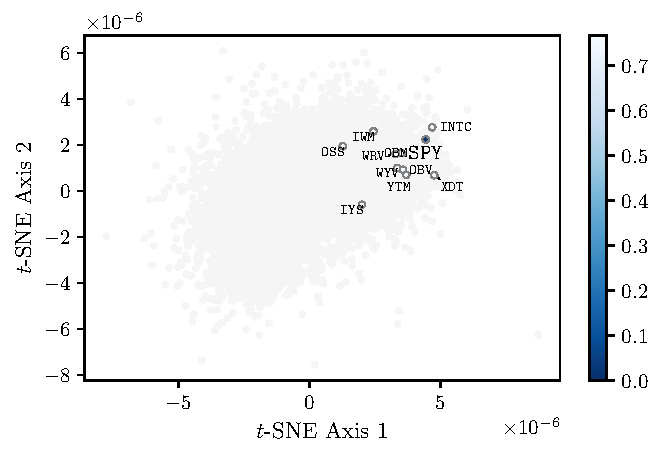
\includegraphics[width=0.6\textwidth]{categorical_embeddings_SPY.pdf}}
    \vfill
    \subfloat[Most Similar Embeddings to $\mathtt{JPM}$\label{fig:fig:cat-embeddings-jpm}]{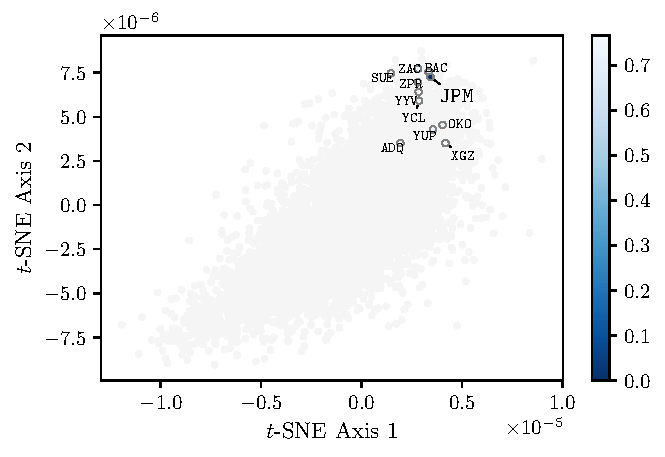
\includegraphics[width=0.6\textwidth]{categorical_embeddings_JPM.pdf}}
    \caption[Categorical Embeddings of Selected Underlyings]{Categorical embeddings of selected underlyings. The plot depicts the projected embedding of SPDR S\&P 500 Trust ($\mathtt{SPY}$) and JPMorgan Chase \& Co ($\mathtt{JPM}$) and their most similar embeddings. Embeddings are projected into 2D-space using $t$-SNE \autocite{vandermaatenVisualizingDataUsing2008}. The ten most similar embeddings by cosine similarity in the original space are coloured and annotated. The model is trained on \gls{ISE} data.}
    \label{fig:categorical-embeddings}
\end{figure}

However, we want to stress the limitations. Both underlyings are among the most frequently traded in our dataset. For infrequent underlyings, embedding are likely close to their random initialisation and hence not meaningful, as no parameter updates take place. The raised problem transfers to handling rare vocabulary items, intensively studied in the context of natural language processing. \todo{Add relevant literature?}

\clearpage

\section{Application in Transaction Cost Estimation}\label{sec:application}

\textbf{Preliminaries}

% TODO: Add why it is important. See Stoll, Huang, Roll (zettelkasten)

Albeit the classification accuracy is a reasonable measure for comparing classifiers, one cannot immediately infer how changes in accuracy e.~g., an improvement by \SI{1}{\percent}, affect the application domains. In an attempt to make our results tangible, we apply all algorithms to estimate trading cost, a problem we previously identified to be reliant on correct trade classification (cp. \cref{sec:introduction}) and a common testing ground for trade classification rules \autocites[cp.][541]{ellisAccuracyTradeClassification2000}[][569]{finucaneDirectTestMethods2000}[][271--278]{petersonEvaluationBiasesExecution2003}[][896--897]{savickasInferringDirectionOption2003}.

One of the most widely adopted measures for trading costs is the effective spread \autocite[][112]{Piwowar_2006}. It is defined as the difference between the trade price and the fundamental value of the asset \autocite[][238--239]{bessembinderIssuesAssessingTrade2003}. Following \textcite[][238--239]{bessembinderIssuesAssessingTrade2003}, we define the \emph{nominal, effective spread} as
\begin{equation}
    S_{i,t} = 2 (P_{i,t} - V_{i,t}) D_{i,t}.
    \label{eq:effective-spread}
\end{equation}

Like before, $i$ indexes the security and $t$ the point in time. Here, $D_{i,t}$ is the trade direction, which is either $1$ for customer buy orders and $-1$ for sell orders. If the trade initiator is known, we set $D_{i,t} = y_{i,t}$ and $D_{i,t}=\hat{y}_{it}$, if inferred from a rule or classifier. As the fundamental value $V_{i,t}$ is unobserved at the time of the trade, we follow a common track in research and use the midpoint of the prevailing quotes as an observable proxy.\footnote{An alternative treatment for options is discussed in \textcite[][4975--4976]{muravyevOptionsTradingCosts2020} Our focus is on the midspread, as it is the most common proxy for the value.} This is also a natural choice, under the assumption that, on average, the spread is symmetric and centred around the true fundamental value \autocite[][1018]{leeMarketIntegrationPrice1993}. We multiply the so-obtained half-spread by $\times 2$ to obtain the effective spread, which represents the cost for a round trip trade involving a buy and sell excluding commissions.

Apparent from \cref{eq:effective-spread}, poor estimates for the predicted trade direction, lead to an under or overestimated effective spread, and hence to a skewed trade cost estimate. Only for trades at the midspread, the predicted trade direction is irrelevant, since the effective spread is zero. By comparing the true effective spread from the estimated, we can derive the economic significance. A classifier correctly classifying every trade, achieves an effective spread estimate equal to the true spread. For a random classifier, the effective spread is around zero, as misclassification estimates the spread with the opposite sign, which offsets with correct, random estimates for other trades.

For convenience, we also calculate the \emph{relative effective spread} as
\begin{equation}
    {PS}_{i,t} = S_{i,t} / V_{i,t}.
\end{equation}
% \todo{check how it is defined Savickas / Finucane use midpoint, Peterson and Sirri divide by price / so does chakrabarty 2007 p. 3819?}

The subsequent section estimates both the nominal and relative effective spread. Following \textcite[][12]{theissenTestAccuracyLee2000} a Wilcoxon test is conducted to assess if the medians of the estimated, effective spread and the true effective spread are equal. The null hypothesis of equal medians is rejected at the \SI{1}{\percent} level.

\textbf{Results}

The actual and the estimated effective spreads for the test sets are shown in the \cref{tab:effective-spread} aggregated by mean. \textcite[][896--897]{savickasInferringDirectionOption2003} estimated the effective spreads of rules on a older subset of option trades at the \gls{CBOE}, which can be compared against. Our results match theirs in magnitude.

\begin{table}[!ht]
    \centering
    \begin{threeparttable}
    \sisetup{
        round-precision = 3, 
      }
    \begin{tabular}{llSSSS}
        \toprule
        {}                                               & {}   & \multicolumn{2}{c}{\gls{ISE}} & \multicolumn{2}{c}{\gls{CBOE}}                                 \\ \cmidrule(lr){3-4}\cmidrule(lr){5-6}
        {Classifier}                                     & {FS} & {Dollar}                      & {Relative}                     & {Dollar} & {Relative}         \\ \midrule
        \multicolumn{6}{l}{Rule-Based}                                                                                                                           \\
        \tabindent $\operatorname{tick}_{\mathrm{ex}}$   & 1    & 0.015534                      & 0.010777 \tnote{*}             & 0.014179 & 0.022880 \tnote{*} \\
        \tabindent $\operatorname{quote}_{\mathrm{ex}}$  & 1    & 0.163333                      & 0.162074 \tnote{*}             & 0.125388 & 0.142093 \tnote{*} \\
        \tabindent $\operatorname{lr}_{\mathrm{ex}}$     & 1    & 0.163333                      & 0.162074 \tnote{*}             & 0.125388 & 0.142093 \tnote{*} \\
        \tabindent $\operatorname{emo}_{\mathrm{ex}}$    & 1    & 0.046443                      & 0.084442 \tnote{*}             & 0.041138 & 0.074176 \tnote{*} \\ 
        \tabindent $\operatorname{clnv}_{\mathrm{ex}}$   & 1    & 0.116247                      & 0.132842 \tnote{*}             & 0.086715 & 0.110510 \tnote{*} \\ 
        \tabindent $\operatorname{gsu}_{\mathrm{small}}$ & 2    & 0.065670                      & 0.096277 \tnote{*}             & 0.084145 & 0.107195 \tnote{*} \\
        \tabindent $\operatorname{gsu}_{\mathrm{large}}$ & 2    & 0.016734                      & 0.044854 \tnote{*}             & 0.053114 & 0.072212 \tnote{*} \\ \midrule
        \multicolumn{6}{l}{Supervised}                                                                                                                           \\
        \tabindent \gls{GBRT}                            & 1    & 0.074294                      & 0.091619 \tnote{*}             & 0.060933 & 0.095318 \tnote{*} \\
        \tabindent \gls{GBRT}                            & 2    & 0.042556                      & 0.069838 \tnote{*}             & 0.036213 & 0.071433 \tnote{*} \\
        \tabindent \gls{GBRT}                            & 3    & 0.039437                      & 0.066473 \tnote{*}             & 0.034674 & 0.066758 \tnote{*} \\ 
        \tabindent  FT-Transformer                       & 2    & 0.030291                      & 0.065596 \tnote{*}             & 0.024942 & 0.063574 \tnote{*} \\
        \tabindent  FT-Transformer                       & 1    & 0.065871                      & 0.086339 \tnote{*}             & 0.057153 & 0.090205 \tnote{*} \\
        \tabindent  FT-Transformer                       & 3    & 0.029874                      & 0.063486 \tnote{*}             & 0.021487 & 0.057358 \tnote{*} \\ \midrule
        \multicolumn{6}{l}{Semi-Supervised}                                                                                                                      \\
        \tabindent \gls{GBRT}                            & 1    & 0.075724                      & 0.092439 \tnote{*}             & 0.065420 & 0.096814 \tnote{*} \\
        \tabindent \gls{GBRT}                            & 2    & 0.043359                      & 0.072062 \tnote{*}             & 0.039600 & 0.073760 \tnote{*} \\
        \tabindent \gls{GBRT}                            & 3    & 0.043240                      & 0.069230 \tnote{*}             & 0.037083 & 0.067946 \tnote{*} \\ 
        \tabindent  FT-Transformer                       & 1    &                               & \tnote{*}                      &          & \tnote{*}          \\
        \tabindent  FT-Transformer                       & 2    &                               & \tnote{*}                      &          & \tnote{*}          \\
        \tabindent  FT-Transformer                       & 3    &                               & \tnote{*}                      &          & \tnote{*}          \\ \midrule
        True Effective Spread                            &      & 0.004926                      & 0.037159                       & 0.012219 & 0.025122           \\ \bottomrule
        % Quoted Spread                                    &      &                                                   &                                                    &          &                 \\ \bottomrule
    \end{tabular}
    \begin{tablenotes}\footnotesize
        \item[*] $p \leq 0.01$.
    \end{tablenotes}
\end{threeparttable}
    \caption{Effective Spreads Estimates of Trade Classification Rules and Classifiers}
    \label{tab:effective-spread}
\end{table}

In summary, quote-based algorithms like the quote rule and the \gls{LR} algorithm severely overestimate the effective spread. The overestimate is less severe for the \gls{CLNV} algorithm due to stronger dependency on the tick rule. The tick rule itself achieves estimates closest to the true effective spread, which is \num[round-mode=places, round-precision=3]{0.004926} and \num[round-mode=places, round-precision=3]{0.012219} for the \gls{ISE} and \gls{CBOE} sample respectively. As primarily tick-based algorithms, like the tick rule or \gls{EMO} rule, perform like a random classifier in our samples, we conclude that the close estimate is an artefact to randomness, not due to superior predictive power. This observation is in line with \textcite[][897]{savickasInferringDirectionOption2003}, who make a similar argument for the \gls{EMO} rule on \gls{CBOE} trades. For rule-based algorithms $\operatorname{gsu}_{\mathrm{large}}$ provides reasonable estimates of the effective spread while achieving high classification accuracy.

From our machine learning-based classifiers the FT-Transformer or \gls{GBRT} trained on FS 3 provides estimates closest to the true effective spread, in particular on the \gls{CBOE} sample. The null hypothesis of equal medians is rejected.

Thus, $\operatorname{gsu}_{\mathrm{large}}$ provides the best estimate of the effective spread if the true labels are absent. For labelled data, Transformer or gradient boosting-based approaches can provide more accurate estimates. The de facto standard, the \gls{LR} algorithm, fails to deliver accurate estimates and may bias empirical research.